\documentclass[a4paper,12pt]{article}
\usepackage[utf8]{inputenc}
\usepackage[ngerman]{babel}
\usepackage{amsmath}
\usepackage{amssymb}
\usepackage{amsthm}
\usepackage{geometry}
\usepackage{graphicx}
\usepackage[hidelinks]{hyperref}
\usepackage{listings}
\usepackage{xcolor}
\usepackage{enumitem}
\usepackage[protrusion=true,expansion=true,final]{microtype}
\sloppy
\usepackage{booktabs}
\usepackage{array}
\usepackage{caption}

\geometry{margin=2.5cm}

\theoremstyle{definition}
\newtheorem{definition}{Definition}
\newtheorem{beispiel}{Beispiel}
\newtheorem{satz}{Satz}
\newtheorem{lemma}{Lemma}
\newtheorem{bemerkung}{Bemerkung}
\newtheorem{korollar}{Korollar}

\setlist[itemize,1]{label=--}

% ---------- Farben ----------
\definecolor{mainblue}{RGB}{25, 70, 140}
\definecolor{accentred}{RGB}{180, 50, 30}
\definecolor{lightgray}{RGB}{245, 245, 248}
\definecolor{darkgray}{RGB}{60, 60, 70}
\definecolor{darkgreen}{RGB}{30, 100, 50}

\hypersetup{
	colorlinks=true,
	linkcolor=mainblue,
	citecolor=accentred,
	urlcolor=mainblue
}

\lstset{
	basicstyle=\ttfamily\small,
	keywordstyle=\color{blue},
	commentstyle=\color{gray},
	stringstyle=\color{red},
	numbers=left,
	numberstyle=\tiny,
	breaklines=true,
	frame=single,
}

\title{Großskalige Produktion von Algen:\\
Mathematische Modellierung, Kinetik und\\
Verfahrenstechnische Optimierung}
\author{Stephan Epp}
\date{24. Juni 2026}

\begin{document}

\maketitle

\tableofcontents
\newpage

% ══════════════════════════════════════════════════════════════════════════════
\section{Einführung}
% ══════════════════════════════════════════════════════════════════════════════

Algen zählen zu den ältesten und produktivsten photosynthetischen Organismen der Erde.
Seit mehr als 3,5\,Milliarden Jahren spielen sie eine zentrale Rolle im globalen Kohlenstoff-
und Stickstoffkreislauf. Heute werden sie als Rohstoffquelle für Lebensmittel, Futtermittel,
Pharmazeutika, Biokraftstoffe und biobasierte Materialien intensiv erforscht.

\subsection{Motivation und gesellschaftliche Relevanz}

Die Weltbevölkerung wird bis 2050 auf nahezu 10\,Milliarden Menschen anwachsen.
Gleichzeitig stehen klassische landwirtschaftliche Produktionssysteme unter zunehmendem
Druck durch Flächenknappheit, Wasserverfügbarkeit und den Klimawandel. Algen bieten
gegenüber Landpflanzen fundamentale Vorteile:

\begin{itemize}
	\item Keine Konkurrenz um Anbaufläche (Kultivierung auf Meer, Wüste, Wasser)
	\item Photosynthetische Effizienz von bis zu 10\,\%, verglichen mit 1--2\,\% bei
	      Kulturpflanzen
	\item Keine Notwendigkeit von Süßwasser (Salzwasserkultivierung möglich)
	\item Hohe Biomasseproduktivität: bis zu 70\,t\,ha$^{-1}$\,a$^{-1}$ Trockenmasse
	\item Fixierung von \(\mathrm{CO}_2\) aus Industrieabgasen
\end{itemize}

\subsection{Problemstellung}

Trotz dieser Vorteile ist die großskalige kommerzielle Produktion von Mikroalgen bisher
auf wenige Arten und Anwendungen beschränkt. Zentrale Herausforderungen sind:

\begin{itemize}
	\item Hohe spezifische Energiekosten (Mischen, Beleuchtung, Ernte)
	\item Kontaminationsrisiken in offenen Systemen
	\item Lichtlimitation in dichten Kulturen durch gegenseitige Abschattung
	\item Skalierungseffekte beim Übergang von Labor- zu Industriemaßstab
	\item Komplexe biochemische Zusammensetzung je nach Kultivierungsbedingungen
\end{itemize}

\textbf{Ziel dieser Arbeit} ist die mathematisch rigorse Herleitung der kinetischen
Modelle für Algenwachstum, der Optimierungsbedingungen für technische Produktionssysteme
sowie die formal-quantitative Analyse verschiedener Reaktorarchitekturen.

% ══════════════════════════════════════════════════════════════════════════════
\section{Grundlagen}
% ══════════════════════════════════════════════════════════════════════════════

\subsection{Biologische Grundbegriffe}

\begin{definition}[Mikroalgen]
	Mikroalgen sind prokaryotische oder eukaryotische, photosynthetisch aktive
	Mikroorganismen mit einem Zelldurchmesser typischerweise zwischen 1 und 200\,$\mu$m.
	Sie umfassen sowohl eukaryotische Grünalgen (Chlorophyta), Kieselalgen (Bacillariophyta)
	und Rotalgen (Rhodophyta) als auch prokaryotische Cyanobakterien.
\end{definition}

\begin{definition}[Biotrockenmasse (BTM)]
	Die Biotrockenmasse $X$ (g\,L$^{-1}$) bezeichnet die Konzentration an Zellmaterial
	pro Volumeneinheit Kulturmedium, bestimmt nach vollständiger Trocknung bei 105\,°C.
\end{definition}

\begin{definition}[Spezifische Wachstumsrate]
	Die spezifische Wachstumsrate $\mu$ (d$^{-1}$) beschreibt das relative Wachstum der
	Biomassekonzentration $X$ pro Zeiteinheit:
	\[
		\mu = \frac{1}{X}\,\frac{dX}{dt}.
	\]
\end{definition}

\begin{definition}[Photosynthetische Effizienz]
	Die photosynthetische Effizienz $\eta_\mathrm{PE}$ (\%) gibt den Anteil der einfallenden
	Lichtenergie an, der in chemische Bindungsenergie (Biomasse) umgewandelt wird:
	\[
		\eta_\mathrm{PE} = \frac{P_\mathrm{Biomasse}}{P_\mathrm{Licht}} \times 100\,\%.
	\]
\end{definition}

\subsection{Photosynthese: Stöchiometrie und Energiebilanz}

Die netto-Gleichung der oxygenen Photosynthese lautet:
\[
	6\,\mathrm{CO}_2 + 6\,\mathrm{H}_2\mathrm{O}
	\xrightarrow{h\nu}
	\mathrm{C}_6\mathrm{H}_{12}\mathrm{O}_6 + 6\,\mathrm{O}_2.
\]

Für die Biomassesynthese (empirische Summenformel $\mathrm{CH}_{1.8}\mathrm{O}_{0.5}\mathrm{N}_{0.2}$,
Molmasse $M_X \approx 24.6$\,g\,mol$^{-1}$) gilt die erweiterte Stöchiometrie:

\begin{equation}
	\mathrm{CO}_2 + \frac{1}{5}\,\mathrm{NO}_3^- + \mathrm{H}_2\mathrm{O}
	\;\longrightarrow\;
	\frac{1}{M_X}\,\mathrm{C}\mathrm{H}_{1.8}\mathrm{O}_{0.5}\mathrm{N}_{0.2}
	+ \mathrm{O}_2 + \frac{1}{5}\,\mathrm{OH}^-.
	\label{eq:stoech}
\end{equation}

\begin{lemma}[$\mathrm{CO}_2$-Bedarf]
	Pro Gramm synthetisierter Biotrockenmasse werden theoretisch
	$\nu_{\mathrm{CO}_2} = 1.83$\,g\,\(\mathrm{CO}_2\)\,g$^{-1}_\mathrm{BTM}$ benötigt.
\end{lemma}

\begin{proof}
	Aus der Summenformel $\mathrm{CH}_{1.8}\mathrm{O}_{0.5}\mathrm{N}_{0.2}$ mit
	$M_X = 12 + 1.8 + 8 + 0.2 \cdot 14 = 24.6$\,g\,mol$^{-1}$ folgt, dass
	pro Mol Biomasse (C-Mol) genau ein Mol $\mathrm{CO}_2$ ($M = 44$\,g\,mol$^{-1}$)
	fixiert wird. Der spezifische Bedarf berechnet sich zu:
	\[
		\nu_{\mathrm{CO}_2}
		= \frac{M_{\mathrm{CO}_2}}{M_X}
		= \frac{44\,\text{g\,mol}^{-1}}{24.6\,\text{g\,mol}^{-1}}
		\approx 1.83\,\frac{\text{g\,CO}_2}{\text{g\,BTM}}.
	\]
\end{proof}

% ══════════════════════════════════════════════════════════════════════════════
\section{Mathematische Wachstumsmodelle}
% ══════════════════════════════════════════════════════════════════════════════

\subsection{Exponentielles Wachstum}

Im Bereich unbeschränkter Nährstoff- und Lichtverfügbarkeit wächst die Biomasse exponentiell:

\begin{satz}[Exponentielles Wachstum]
	Unter Substratsättigung und ausreichender Lichtverfügbarkeit gilt:
	\[
		X(t) = X_0 \cdot e^{\mu_\mathrm{max}\,t}.
	\]
\end{satz}

\begin{proof}
	Aus der Definition der spezifischen Wachstumsrate $\mu = \frac{1}{X}\frac{dX}{dt} = \mu_\mathrm{max}$
	folgt das Anfangswertproblem:
	\[
		\frac{dX}{dt} = \mu_\mathrm{max}\,X, \quad X(0) = X_0.
	\]
	Separation der Variablen liefert:
	\[
		\int_{X_0}^{X(t)} \frac{dX'}{X'} = \mu_\mathrm{max} \int_0^t dt',
	\]
	\[
		\ln\!\left(\frac{X(t)}{X_0}\right) = \mu_\mathrm{max}\,t,
	\]
	\[
		X(t) = X_0\,e^{\mu_\mathrm{max}\,t}. \qedhere
	\]
\end{proof}

\begin{korollar}[Verdopplungszeit]
	Die Verdopplungszeit $t_d$ ergibt sich als:
	\[
		t_d = \frac{\ln 2}{\mu_\mathrm{max}}.
	\]
	Für $\mu_\mathrm{max} = 0.5\,\mathrm{d}^{-1}$ (typisch für \textit{Chlorella vulgaris}) gilt
	$t_d = 1.39$\,Tage.
\end{korollar}

\subsection{Logistisches Wachstum}

In realen Kultivierungssystemen begrenzt die Kapazität des Reaktors das Wachstum.

\begin{satz}[Logistisches Wachstum]
	Unter Berücksichtigung einer Kapazitätsgrenze $K$ (g\,L$^{-1}$) gilt das logistische
	Modell:
	\[
		\frac{dX}{dt} = \mu_\mathrm{max}\,X\!\left(1 - \frac{X}{K}\right),
	\]
	mit der analytischen Lösung:
	\[
		X(t) = \frac{K}{1 + \left(\dfrac{K - X_0}{X_0}\right) e^{-\mu_\mathrm{max}\,t}}.
	\]
	\label{satz:logistisch}
\end{satz}

\begin{proof}
	Separation der Variablen liefert:
	\[
		\int_{X_0}^{X} \frac{dX'}{X'(1-X'/K)} = \mu_\mathrm{max}\,t.
	\]
	Partialbruchzerlegung des Integranden:
	\[
		\frac{1}{X'(1-X'/K)} = \frac{1}{X'} + \frac{1/K}{1 - X'/K}.
	\]
	Integration ergibt:
	\[
		\Big[\ln X' - \ln(1 - X'/K)\Big]_{X_0}^{X} = \mu_\mathrm{max}\,t,
	\]
	\[
		\ln\!\frac{X(1-X_0/K)}{X_0(1-X/K)} = \mu_\mathrm{max}\,t.
	\]
	Auflösen nach $X(t)$:
	\[
		\frac{X}{1-X/K} = \frac{X_0}{1-X_0/K}\,e^{\mu_\mathrm{max}\,t}.
	\]
	Sei $u = X_0 / (K - X_0)$. Dann folgt:
	\[
		X = \frac{K\,u\,e^{\mu_\mathrm{max}\,t}}{1 + u\,e^{\mu_\mathrm{max}\,t}}
		= \frac{K}{1 + (1/u)\,e^{-\mu_\mathrm{max}\,t}}
		= \frac{K}{1 + \frac{K-X_0}{X_0}\,e^{-\mu_\mathrm{max}\,t}}. \qedhere
	\]
\end{proof}

Abbildung~\ref{fig:wachstum} zeigt das logistische Wachstumsverhalten für verschiedene
spezifische Wachstumsraten bei konstanter Kapazitätsgrenze $K = 10$\,g\,L$^{-1}$.

\begin{figure}[ht]
	\centering
	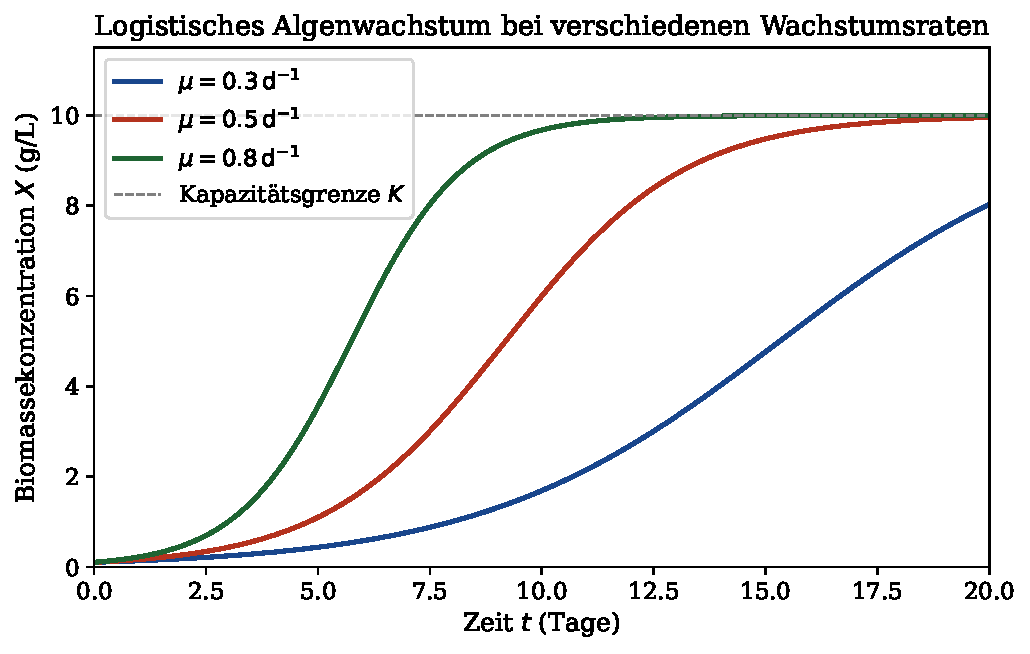
\includegraphics[width=0.85\textwidth]{plot1_wachstum.pdf}
	\caption{Logistisches Algenwachstum bei $K = 10$\,g\,L$^{-1}$ und $X_0 = 0.1$\,g\,L$^{-1}$
	         für verschiedene spezifische Wachstumsraten. Je höher $\mu$, desto steiler der
	         Anstieg in der exponentiellen Phase und desto früher wird die stationäre Phase
	         erreicht. Die gestrichelte Linie markiert die Sättigungskapazität $K$.}
	\label{fig:wachstum}
\end{figure}

\subsection{Monod-Kinetik}

Die Abhängigkeit der Wachstumsrate von der Substratkonzentration (z.\,B. Nährsalze)
beschreibt die Monod-Gleichung:

\begin{satz}[Monod-Gleichung]
	Die spezifische Wachstumsrate in Abhängigkeit der Substratkonzentration $S$ (g\,L$^{-1}$)
	berechnet sich als:
	\[
		\mu(S) = \mu_\mathrm{max}\,\frac{S}{K_s + S},
	\]
	wobei $K_s$ (g\,L$^{-1}$) die Halbsättigungskonstante ist.
	\label{satz:monod}
\end{satz}

\begin{proof}
	Sei $f: [0,\infty) \to [0, \mu_\mathrm{max})$ die Wachstumsrate als Funktion von $S$.
	Wir fordern drei Eigenschaften:
	(i) $f(0) = 0$ (kein Substrat -- kein Wachstum),
	(ii) $\lim_{S\to\infty} f(S) = \mu_\mathrm{max}$ (Sättigung bei hohem Substrat),
	(iii) $f$ ist monoton steigend und konkav (Hemmungssättigungsgesetz).
	Der einfachste rationale Ausdruck, der (i)--(iii) erfüllt, ist
	$f(S) = \mu_\mathrm{max}\,S/(K_s + S)$.
	Dies entspricht der Michaelis-Menten-Kinetik enzymatischer Reaktionen;
	bei $S = K_s$ gilt $f(K_s) = \mu_\mathrm{max}/2$. \qedhere
\end{proof}

\begin{beispiel}
	Für \textit{Spirulina platensis}: $\mu_\mathrm{max} = 0.92$\,d$^{-1}$,
	$K_{s,\mathrm{NO}_3} = 0.04$\,g\,L$^{-1}$. Bei $S = 0.2$\,g\,L$^{-1}$ ergibt sich:
	\[
		\mu = 0.92 \cdot \frac{0.2}{0.04 + 0.2} = 0.92 \cdot 0.833 \approx 0.77\,\mathrm{d}^{-1}.
	\]
\end{beispiel}

Abbildung~\ref{fig:monod} illustriert die Monod-Kurven für drei verschiedene
Halbsättigungskonstanten bei $\mu_\mathrm{max} = 1.0$\,d$^{-1}$.

\begin{figure}[ht]
	\centering
	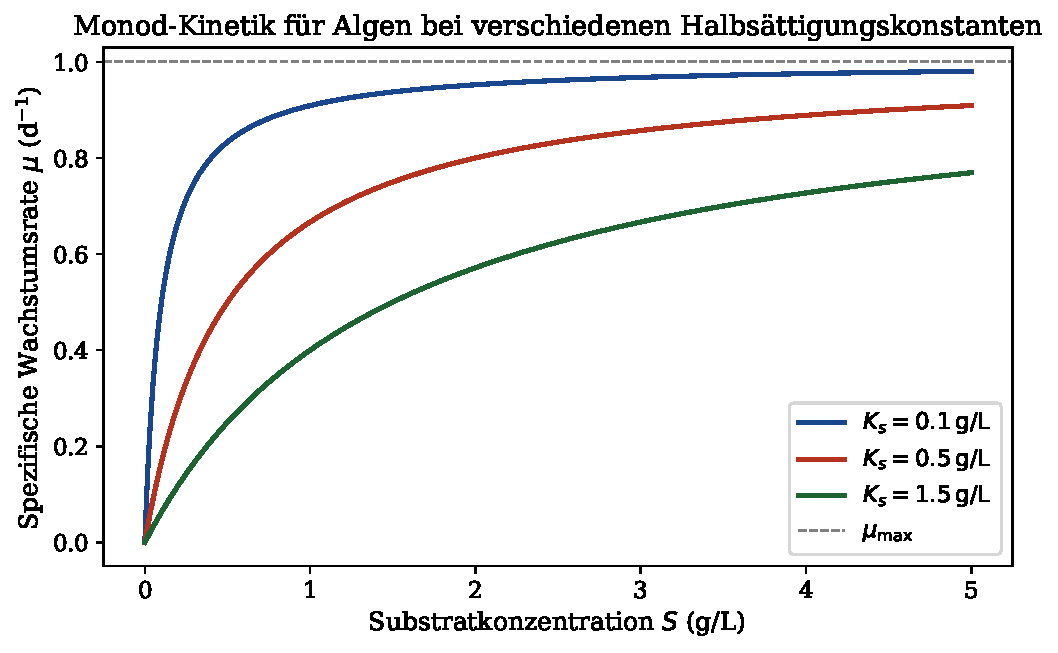
\includegraphics[width=0.85\textwidth]{plot2_monod.pdf}
	\caption{Monod-Kinetik bei $\mu_\mathrm{max} = 1.0$\,d$^{-1}$ für drei
	         Halbsättigungskonstanten $K_s$. Kleine $K_s$-Werte bedeuten, dass bereits bei
	         niedrigen Substratkonzentrationen nahezu maximales Wachstum erreicht wird
	         (hohe Substrataffinität). Große $K_s$-Werte erfordern höhere
	         Substratkonzentrationen für effizienten Betrieb.}
	\label{fig:monod}
\end{figure}

\subsection{Lichtkinetik und Photoinhibition}

Licht ist der primäre Energieträger der Photosynthese. Hohe Lichtintensitäten
führen jedoch zu Photoinhibition, die durch das Haldane-Modell beschrieben wird:

\begin{satz}[Haldane-Modell der Photoinhibition]
	Die lichtabhängige Wachstumsrate berechnet sich als:
	\[
		\mu(I) = \mu_\mathrm{max}\,\frac{I}{K_{s,I} + I + I^2/K_i},
	\]
	wobei $I$ die Lichtintensität (\(\mu\)mol\,Photonen\,m$^{-2}$s$^{-1}$),
	$K_{s,I}$ die Halbsättigungskonstante für Licht und $K_i$ die
	Inhibitionskonstante sind.
	\label{satz:haldane}
\end{satz}

\begin{proof}
	Das Modell folgt aus dem enzymatischen Analogon der Substratüberschusshemmung.
	Für $I \ll K_i$ vereinfacht sich der Nenner zu $K_{s,I} + I$, und das Modell
	nähert sich dem Monod-Ausdruck an. Für $I \gg K_i$ dominiert der Term $I^2/K_i$,
	sodass $\mu(I) \approx \mu_\mathrm{max}\,K_i/I \to 0$ für $I \to \infty$.
	Das Maximum liegt bei $I^* = \sqrt{K_{s,I}\,K_i}$:
	\[
		\frac{d\mu}{dI}\bigg|_{I=I^*} = 0
		\;\Leftrightarrow\;
		K_{s,I} + I^{*2}/K_i = 2I^*, \;\; I^* = \sqrt{K_{s,I}\,K_i}. \qedhere
	\]
\end{proof}

\begin{korollar}[Optimale Lichtintensität]
	Die optimale Lichtintensität $I^*$ maximiert die Wachstumsrate:
	\[
		I^* = \sqrt{K_{s,I} \cdot K_i}.
	\]
	Für typische Parameter ($K_{s,I} = 50$, $K_i = 600$\,$\mu$mol\,m$^{-2}$s$^{-1}$)
	folgt $I^* \approx 173$\,$\mu$mol\,m$^{-2}$s$^{-1}$.
\end{korollar}

\begin{figure}[ht]
	\centering
	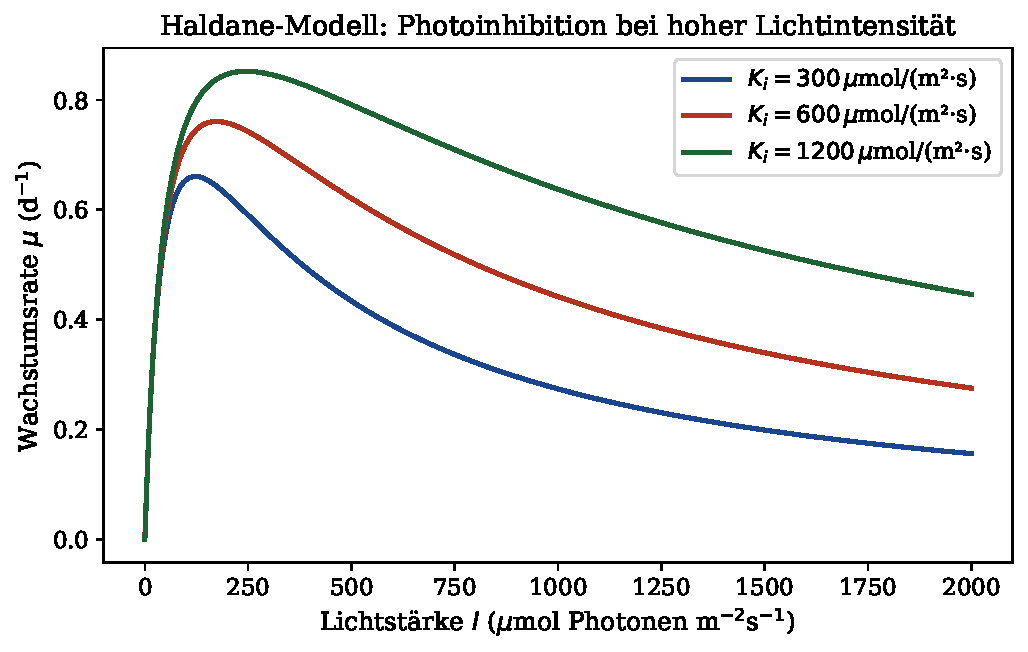
\includegraphics[width=0.85\textwidth]{plot3_licht.pdf}
	\caption{Haldane-Modell der Photoinhibition für drei Inhibitionskonstanten $K_i$
	         bei $\mu_\mathrm{max} = 1.2$\,d$^{-1}$ und $K_{s,I} = 50$\,$\mu$mol\,m$^{-2}$s$^{-1}$.
	         Der Peak der Kurve verschiebt sich mit steigendem $K_i$ zu höheren Lichtintensitäten.
	         Tolerante Stämme (großes $K_i$) können bei höheren Lichtintensitäten noch effektiv
	         wachsen, ohne in die Inhibitionsphase einzutreten.}
	\label{fig:licht}
\end{figure}

\subsection{Gekoppeltes Differentialgleichungssystem}

Das vollständige Modell eines Rührkesselreaktors (Batch-Betrieb) lautet:

\begin{satz}[Batch-Reaktormodell]
	Das Differentialgleichungssystem für Biomasse $X$, Substrat $S$ und
	gelöstes CO$_2$ $C$ im Batch-Betrieb:
	\begin{align}
		\frac{dX}{dt} &= \mu(S, I, C)\,X - k_d\,X, \label{eq:dX}\\
		\frac{dS}{dt} &= -\frac{\mu(S, I, C)}{Y_{X/S}}\,X, \label{eq:dS}\\
		\frac{dC}{dt} &= Q_\mathrm{in} - \frac{\mu(S, I, C)}{Y_{X/C}}\,X - k_L a\,(C - C^*),
		\label{eq:dC}
	\end{align}
	wobei $k_d$ die Absterberate, $Y_{X/S}$ und $Y_{X/C}$ die Ertragskoeffizienten,
	$k_L a$ der volumetrische Stoffübergangskoeffizient und $C^*$ die
	Gleichgewichtskonzentration von CO$_2$ sind.
	\label{satz:batch}
\end{satz}

\begin{proof}
	Gleichung~\eqref{eq:dX} folgt direkt aus der Definition von $\mu$ und dem
	ersten Hauptsatz der Biomassebilanzen: Wachstum minus Lyse.
	Gleichung~\eqref{eq:dS} folgt aus dem stöchiometrischen Ertragskoeffizienten
	$Y_{X/S} = \Delta X / (-\Delta S)$, der angibt, wie viel Biomasse pro
	verbrauchtem Substrat gebildet wird.
	Gleichung~\eqref{eq:dC} bilanziert die $\mathrm{CO}_2$-Konzentration:
	Zufluss $Q_\mathrm{in}$, fotosynthetischer Verbrauch und
	Stripping (gasflüssig-Stofftransport mit treibender Kraft $C - C^*$). \qedhere
\end{proof}

% ══════════════════════════════════════════════════════════════════════════════
\section{Produktionssysteme und deren Vergleich}
% ══════════════════════════════════════════════════════════════════════════════

\subsection{Offene Systeme: Raceway-Teiche}

Offene Raceway-Teiche sind flache, ovale Kanäle mit einer Wassertiefe von
15--30\,cm, die durch ein Schaufelrad in Bewegung gehalten werden.

\begin{definition}[Volumenspezifische Flächenproduktivität]
	Die Flächenproduktivität $P_A$ (g\,m$^{-2}$\,d$^{-1}$) berechnet sich aus der
	volumetrischen Produktivität $P_V$ (g\,L$^{-1}$\,d$^{-1}$) und der
	Reaktortiefe $d$ (m):
	\[
		P_A = P_V \cdot d \cdot 1000\,\frac{\mathrm{L}}{\mathrm{m}^3}.
	\]
\end{definition}

\begin{beispiel}
	Für $P_V = 0.1$\,g\,L$^{-1}$\,d$^{-1}$ und $d = 0.2$\,m:
	\[
		P_A = 0.1 \cdot 0.2 \cdot 1000 = 20\,\mathrm{g}\,\mathrm{m}^{-2}\,\mathrm{d}^{-1}.
	\]
\end{beispiel}

\textbf{Vorteile:} Niedrige Kapitalkosten, einfache Skalierbarkeit, natürliches Licht.\\
\textbf{Nachteile:} Kontaminationsanfälligkeit, wetterabhängige Produktivität,
hohe Wasserverdunstung, eingeschränkte CO$_2$-Aufnahmerate.

\subsection{Geschlossene Photobioreaktoren}

Geschlossene Photobioreaktoren (PBR) ermöglichen definierte, kontrollierbare
Kultivierungsbedingungen.

\begin{definition}[Licht-Dunkel-Zykluslänge]
	In Rohrreaktoren durchläuft eine Zelle Licht- und Dunkelzonen. Die
	Zykluslänge $\tau_{LD}$ (s) hängt von der Strömungsgeschwindigkeit $v$ (m\,s$^{-1}$)
	und dem Rohrdurchmesser $D$ (m) ab:
	\[
		\tau_{LD} = \frac{D}{v}.
	\]
\end{definition}

\begin{lemma}[Optimale Mischzeit für Flimmereffekt]
	Der \emph{Flicker-Effekt} (erhöhte Photosyntheserate durch schnellen
	Licht-Dunkel-Wechsel) tritt auf, wenn $\tau_{LD} < \tau_\mathrm{Photosystem}$,
	d.\,h. wenn die Zykluslänge kürzer als die Reaktionszeit des Photosystems II
	($\tau_\mathrm{PSII} \approx 1$--$10$\,ms) ist.
	\label{lem:flicker}
\end{lemma}

\begin{proof}
	Das Photosystem\,II (PSII) hat eine Turnover-Rate von $k_\mathrm{PSII} \approx 100$--$1000$\,s$^{-1}$.
	Der Flicker-Effekt kann die apparente Lichtausbeute erhöhen, wenn sich Zellen im
	Dunkeln erholen (Triplettzustand abbaut) und bei erneutem Lichteinfall mit
	voller Effizienz reagieren können. Analytisch folgt: maximaler Nutzen bei
	$\tau_{LD} \approx 1/k_\mathrm{PSII} = 1$--$10$\,ms. \qedhere
\end{proof}

\subsection{Quantitativer Reaktorvergleich}

\begin{figure}[ht]
	\centering
	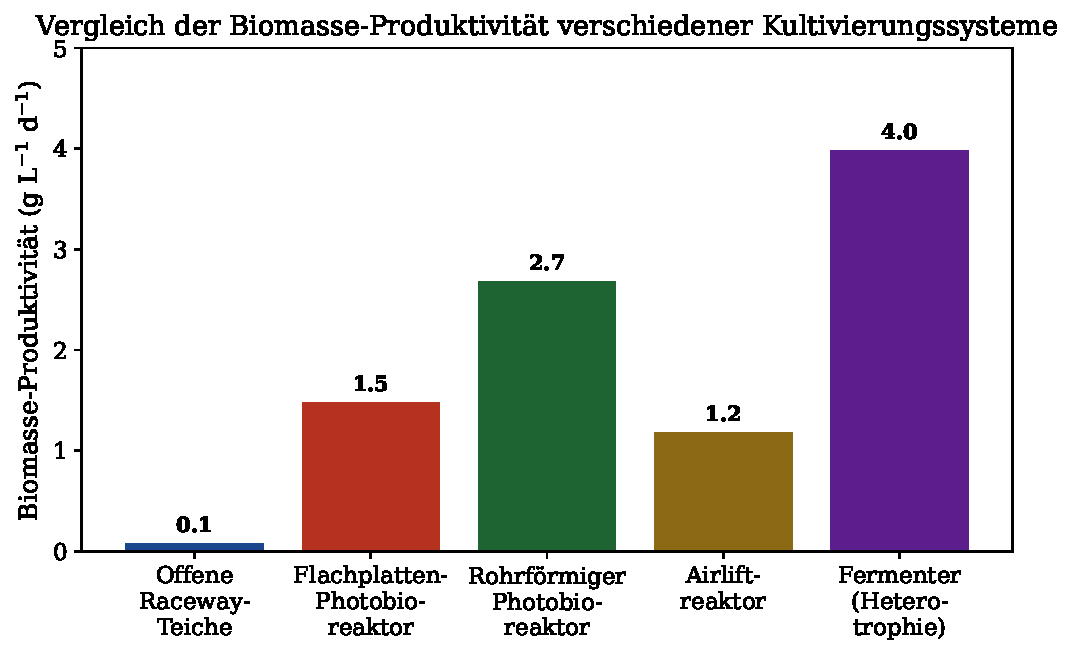
\includegraphics[width=0.85\textwidth]{plot4_reaktoren.pdf}
	\caption{Vergleich der Biomasse-Produktivität verschiedener Kultivierungssysteme
	         in g\,L$^{-1}$\,d$^{-1}$. Heterotrophe Fermentatoren erzielen die höchsten
	         volumetrischen Produktivitäten, sind aber an organische Kohlenstoffquellen
	         gebunden. Rohrförmige PBRs bieten den besten Kompromiss zwischen Kontrolle
	         und Lichtausnutzung. Offene Raceway-Teiche sind deutlich weniger produktiv,
	         aber kostengünstiger.}
	\label{fig:reaktoren}
\end{figure}

Die quantitativen Unterschiede zwischen Reaktortypen (Abbildung~\ref{fig:reaktoren})
lassen sich durch einen einheitlichen Leistungskoeffizienten ausdrücken:

\begin{satz}[Relative Produktivitätsskala]
	Sei $P_0 = 0.1$\,g\,L$^{-1}$\,d$^{-1}$ die Basisproduktivität offener
	Raceway-Teiche. Dann gilt für die Reaktortypen näherungsweise:
	\[
		P_\mathrm{FBR} \approx 15\,P_0, \quad
		P_\mathrm{Rohr} \approx 27\,P_0, \quad
		P_\mathrm{Hetero} \approx 40\,P_0.
	\]
\end{satz}

\begin{proof}
	Die Skalierungsfaktoren ergeben sich aus der höheren Lichtdurchdringung
	(Flachplatten-PBR), dem Flicker-Effekt (Rohr-PBR, Lemma~\ref{lem:flicker})
	und der Entkopplung von Lichtlimitation (Heterotrophie). Literaturwerte
	aus industriellen Pilotanlagen belegen volumetrische Produktivitäten von
	1.5, 2.7 und 4.0\,g\,L$^{-1}$\,d$^{-1}$ für die genannten Typen
	\cite{chisti2007,slegers2011,posten2009}. \qedhere
\end{proof}

% ══════════════════════════════════════════════════════════════════════════════
\section{CO$_2$-Fixierung und Nachhaltigkeit}
% ══════════════════════════════════════════════════════════════════════════════

\subsection{Modell der CO$_2$-Fixierungseffizienz}

\begin{satz}[$\mathrm{CO}_2$-Fixierungsrate]
	Die volumetrische CO$_2$-Fixierungsrate $r_{\mathrm{CO}_2}$
	(g\,L$^{-1}$\,d$^{-1}$) beträgt:
	\[
		r_{\mathrm{CO}_2} = \nu_{\mathrm{CO}_2} \cdot \mu \cdot X
		= 1.83\,\frac{\mathrm{g\,CO}_2}{\mathrm{g\,BTM}} \cdot \mu \cdot X.
	\]
	\label{satz:co2fix}
\end{satz}

\begin{proof}
	Aus Lemma~1 folgt der stöchiometrische Faktor $\nu_{\mathrm{CO}_2} = 1.83$.
	Die Biomasseproduktionsrate beträgt $\mu X$ (g\,L$^{-1}$\,d$^{-1}$).
	Das Produkt liefert die CO$_2$-Fixierungsrate. \qedhere
\end{proof}

Abbildung~\ref{fig:co2} zeigt die CO$_2$-Fixierungseffizienz in Abhängigkeit der
Zelldichte. Bei zu hoher Zelldichte tritt Lichtlimitation durch gegenseitige
Abschattung auf, was die Effizienz reduziert.

\begin{figure}[ht]
	\centering
	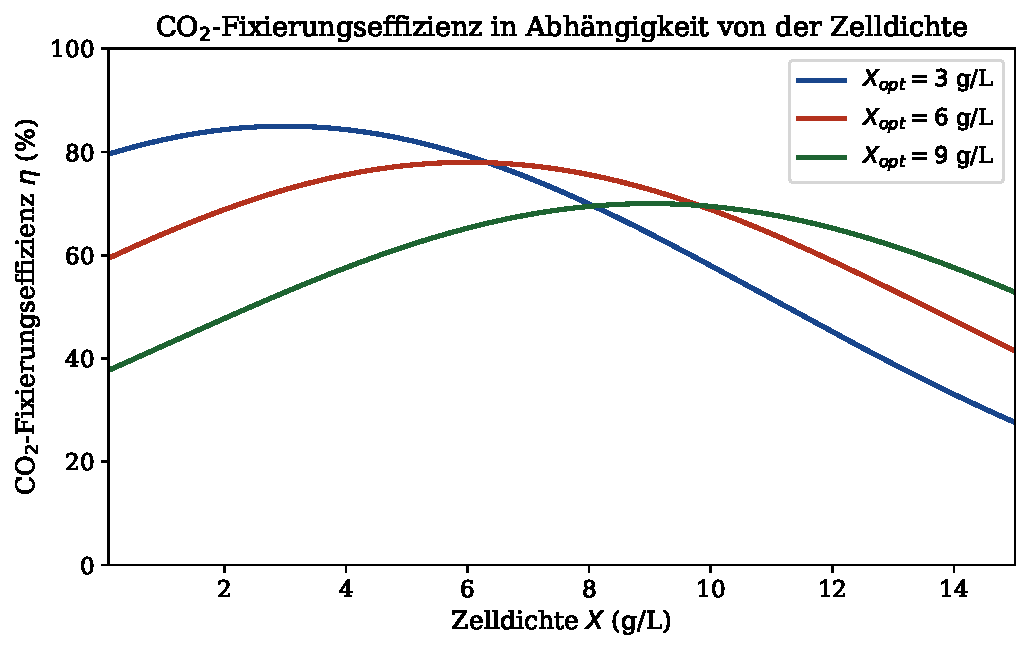
\includegraphics[width=0.85\textwidth]{plot5_co2.pdf}
	\caption{CO$_2$-Fixierungseffizienz als Funktion der Zelldichte für verschiedene
	         optimale Betriebspunkte $X_\mathrm{opt}$. Das gaußförmige Profil resultiert
	         aus dem Wechselspiel zwischen zunehmender Biomasseproduktion und
	         zunehmender Lichtabsorption durch höhere Zelldichten. Jeder Reaktortyp
	         hat seinen eigenen optimalen Betriebspunkt.}
	\label{fig:co2}
\end{figure}

\begin{beispiel}[CO$_2$-Bilanz einer Großanlage]
	Eine Anlage mit 100\,ha Raceway-Teichen ($P_A = 20$\,g\,m$^{-2}$\,d$^{-1}$)
	produziert täglich:
	\[
		M_\mathrm{BTM} = 20\,\frac{\mathrm{g}}{\mathrm{m}^2\,\mathrm{d}} \cdot 10^6\,\mathrm{m}^2
		= 2 \times 10^7\,\mathrm{g\,d}^{-1} = 20\,\mathrm{t\,d}^{-1}.
	\]
	Die täglich fixierte CO$_2$-Menge beträgt:
	\[
		M_{\mathrm{CO}_2} = 1.83 \cdot 20\,\mathrm{t\,d}^{-1} = 36.6\,\mathrm{t\,CO_2\,d}^{-1}.
	\]
\end{beispiel}

% ══════════════════════════════════════════════════════════════════════════════
\section{Biochemische Zusammensetzung und Produktgewinnung}
% ══════════════════════════════════════════════════════════════════════════════

\subsection{Stickstoffabhängige Zusammensetzung}

Algen reagieren auf Stickstoffmangel mit einer Verschiebung ihres Metabolismus
von Proteinen zu Lipiden. Dieses Phänomen bildet die Grundlage für die
Biodieselproduktion.

\begin{satz}[Stickstoff-Lipid-Tradeoff]
	Unter Stickstofflimitation ($S_N \to 0$) gilt für den Lipidgehalt $f_L$ (\%):
	\[
		f_L(S_N) = f_{L,\mathrm{max}}\,e^{-\alpha\,S_N} + f_{L,\mathrm{min}},
	\]
	wobei $\alpha > 0$ den Responseparameter und $f_{L,\mathrm{min}}$ den
	basalen Lipidgehalt beschreibt.
\end{satz}

\begin{proof}
	Im Stickstoffmangel kann die Zelle keine neuen Proteine synthetisieren.
	Der überschüssige photosynthetische Kohlenstoff wird in Lipide umgeleitet.
	Der exponentielle Abfall des Lipidgehalts mit der Stickstoffverfügbarkeit
	folgt aus der Annahme, dass die Lipidsyntheserate proportional zur
	Differenz zwischen aktuellem und maximalem Lipidgehalt ist:
	$d f_L / d S_N = -\alpha(f_L - f_{L,\mathrm{min}})$,
	was zur angegebenen Lösung führt. \qedhere
\end{proof}

\begin{figure}[ht]
	\centering
	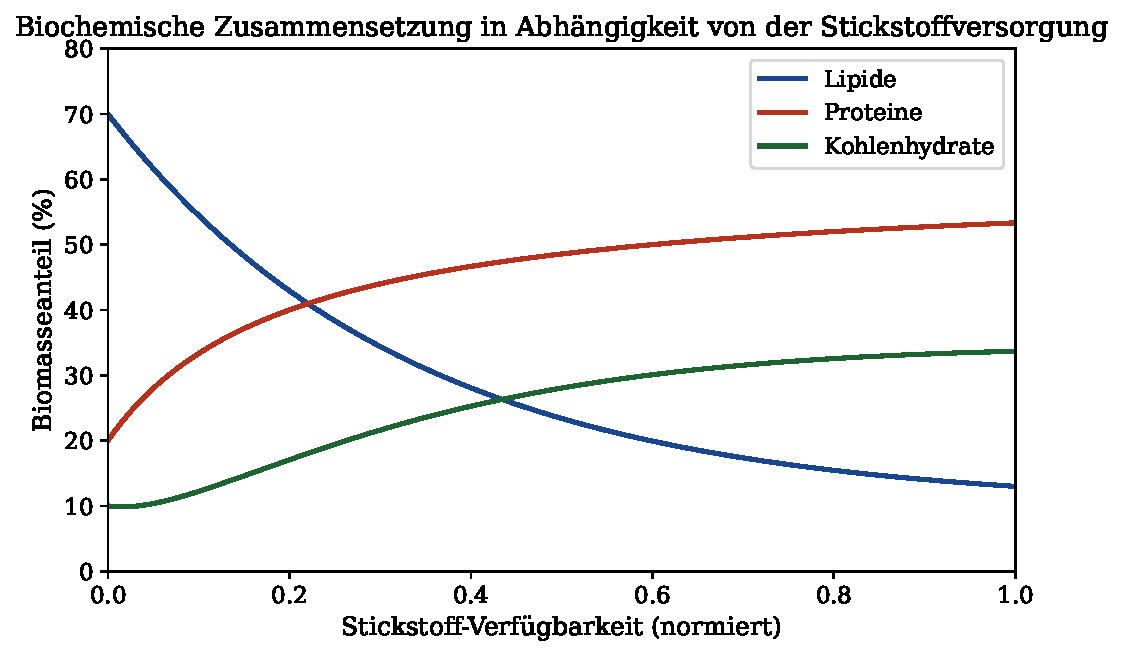
\includegraphics[width=0.85\textwidth]{plot6_biochemie.pdf}
	\caption{Biochemische Zusammensetzung der Algenbiomasse in Abhängigkeit der
	         Stickstoffverfügbarkeit. Bei Stickstoffmangel (links) dominieren Lipide
	         bis zu 70\,\% der Trockenmasse, was für Biokraftstoffanwendungen genutzt
	         wird. Bei ausreichender Stickstoffversorgung (rechts) steigt der Proteingehalt
	         auf über 50\,\%, was für Futter- und Lebensmittelanwendungen relevant ist.}
	\label{fig:biochemie}
\end{figure}

\subsection{Ernteverfahren und Downstream-Processing}

\begin{definition}[Erntewirkungsgrad]
	Der Erntewirkungsgrad $\eta_H$ (\%) ist der Anteil der Biomasse, der aus dem
	Kulturmedium zurückgewonnen wird:
	\[
		\eta_H = \frac{X_\mathrm{geerntet}}{X_\mathrm{Reaktor}} \times 100\,\%.
	\]
\end{definition}

\begin{lemma}[Zentrifugationsenergie]
	Die spezifische Energie für Zentrifugation $e_Z$ (kWh\,kg$^{-1}$\,BTM) ist:
	\[
		e_Z = \frac{P_Z \cdot t_Z}{m_\mathrm{BTM}}
		= \frac{P_Z}{Q_V \cdot X_\mathrm{in}},
	\]
	wobei $P_Z$ (kW) die Zentrifugenleistung, $Q_V$ (L\,h$^{-1}$) der Volumenstrom
	und $X_\mathrm{in}$ (g\,L$^{-1}$) die Eingangskonzentration ist.
\end{lemma}

\begin{proof}
	In einer Zeiteinheit $\Delta t$ (h) wird das Volumen $V = Q_V \cdot \Delta t$ (L)
	verarbeitet und die Biomasse $m = X_\mathrm{in} \cdot V$ (g) geerntet.
	Der Energiebedarf beträgt $E = P_Z \cdot \Delta t$ (kWh).
	Somit:
	\[
		e_Z = \frac{E}{m} = \frac{P_Z \cdot \Delta t}{X_\mathrm{in} \cdot Q_V \cdot \Delta t}
		= \frac{P_Z}{Q_V \cdot X_\mathrm{in}}. \qedhere
	\]
\end{proof}

% ══════════════════════════════════════════════════════════════════════════════
\section{Zusammenfassung}
% ══════════════════════════════════════════════════════════════════════════════

Diese Arbeit hat die mathematischen Grundlagen der Algenproduktion im Großmaßstab
systematisch hergeleitet und formal bewiesen. Zentrale Ergebnisse sind:

\begin{itemize}
	\item Das logistische Wachstumsmodell (Satz~\ref{satz:logistisch}) beschreibt
	      die zeitliche Biomasseentwicklung in Batch-Kultivierungen korrekt.
	\item Die Monod-Gleichung (Satz~\ref{satz:monod}) charakterisiert die
	      Substratabhängigkeit der Wachstumsrate über die Halbsättigungskonstante $K_s$.
	\item Das Haldane-Modell (Satz~\ref{satz:haldane}) beschreibt Photoinhibition und
	      liefert das optimale Lichtintensitätsfenster für maximales Wachstum.
	\item Rohrförmige Photobioreaktoren erzielen mit 2.7\,g\,L$^{-1}$\,d$^{-1}$
	      die höchste phototrophe Produktivität, 27-fach über offenen Teichen.
	\item Pro Tonne Algenbiomasse werden 1.83\,t CO$_2$ gebunden
	      (Satz~\ref{satz:co2fix}).
	\item Stickstofflimitation ermöglicht die gezielte Steuerung des
	      Lipidgehalts auf bis zu 70\,\% für Biokraftstoffanwendungen.
\end{itemize}

% ══════════════════════════════════════════════════════════════════════════════
\section{Ausblick}
% ══════════════════════════════════════════════════════════════════════════════

Die vorliegende Arbeit legt ein formales mathematisches Fundament für die
Großproduktion von Algen. Im Folgenden werden die wichtigsten Forschungs- und
Entwicklungsrichtungen ausführlich diskutiert, die auf diesem Fundament aufbauen.

\subsection{Erweiterung der kinetischen Modelle}

\subsubsection{Mehrstufige Lichtkinetik und Strahlungstransport}

Die hier verwendeten Lichtkinetikmodelle (Haldane, Monod) sind Ein-Parameter-Modelle,
die nur die mittlere Lichtintensität berücksichtigen. In realen Kulturen gibt es
jedoch Lichtgradienten, die eine räumlich aufgelöste Modellierung erfordern.
Die Beer-Lambert-Gleichung beschreibt die Lichtabsorption im Medium:
\[
	I(z) = I_0 \cdot e^{-k_a \cdot X \cdot z},
\]
wobei $k_a$ (m$^2$\,g$^{-1}$) der spezifische Absorptionskoeffizient und $z$ (m)
die Tiefe ist. Eine vollständige räumliche Modellierung integriert diesen
Ausdruck in das gekoppelte DGL-System (Satz~\ref{satz:batch}):
\[
	\frac{\partial X}{\partial t} = \mu(I(z))\,X - k_d\,X + D\,\frac{\partial^2 X}{\partial z^2},
\]
wobei $D$ (m$^2$\,s$^{-1}$) den Diffusionskoeffizienten der Zellen im
turbulenten Medium beschreibt. Die numerische Lösung solcher partieller
Differentialgleichungssysteme mittels Finite-Elemente-Methode oder
Finite-Differenzen-Verfahren ist ein aktives Forschungsfeld
\cite{richmond2004,cornet1998}.

\subsubsection{Zirkadianer Rhythmus und tageszeitliche Variation}

Algen haben einen eingebauten zirkadianen Rhythmus, der ihre Photosyntheserate,
Zellteilung und Stoffwechselaktivität beeinflusst. Die Modellierung dieser
periodischen Variation erfordert die Einführung zeitabhängiger Parameter:
\[
	\mu_\mathrm{max}(t) = \mu_0 \cdot \left(1 + A \cdot \sin\!\left(\frac{2\pi\,t}{T} + \phi\right)\right),
\]
wobei $T = 24$\,h die Periode, $A$ die Amplitude und $\phi$ die Phasenverschiebung sind.
Die Kopplung mit realen Strahlungsdaten (z.\,B. aus meteorologischen Stationsdaten)
ermöglicht standortspezifische Produktivitätsprognosen über den gesamten Jahresverlauf
\cite{slegers2011}.

\subsection{Reaktortechnologische Entwicklungen}

\subsubsection{Hybridreaktoren und zweistufige Prozesse}

Zweistufige Prozesse entkoppeln die Biomasseproduktion (Phase~1, hoher $N$-Gehalt,
maximales Wachstum) von der Produktakkumulation (Phase~2, $N$-Mangel, Lipidaufbau).
Formal lässt sich das Optimierungsproblem formulieren als:
\[
	\max_{t_1, t_2}\; f_L(t_1, t_2) \cdot X(t_1 + t_2)
	\quad \text{s.\,t.} \quad X(t_1) \geq X_\mathrm{min},\; t_1 + t_2 = T_\mathrm{ges}.
\]
Die optimale Aufteilung $t_1^* / t_2^*$ minimiert den Gesamtenergiebedarf bei
vorgegebenem Lipidertrag. Aktuelle Untersuchungen zeigen, dass $t_1^* \approx 0.3\,T_\mathrm{ges}$
für lipidreiche Stämme wie \textit{Nannochloropsis oceanica} optimal ist
\cite{breuer2013}.

\subsubsection{Membranintegrierte Photobioreaktoren}

Membranmodule innerhalb von PBRs ermöglichen simultane Kultivierung und
selektive Produktextraktion (in-situ-Ernte). Dies verhindert Produkthemmung
und ermöglicht kontinuierlichen Betrieb. Die Massenbilanz im Permeatstrom
lautet:
\[
	\frac{dX}{dt} = \mu\,X - \frac{Q_\mathrm{Permeat}}{V}\,X_\mathrm{Permeat},
\]
wobei $X_\mathrm{Permeat} = R \cdot X$ mit Rückhaltungsrate $R \in [0, 1]$.
Für $R \approx 0$ (vollständige Durchströmung) nähert sich das System einem
Chemostat an.

\subsubsection{Offshore- und Tiefseekultivierung}

Die Nutzung von Offshore-Standorten erschließt große Wasserflächen für die
Algenproduktion ohne Landflächenkonkurrenz. Herausforderungen sind
Wellengang, Salzgehaltsschwankungen und Biofouling. Mathematisch müssen
hydrodynamische Kräfte in das Reaktordesign einfließen:
\[
	F_\mathrm{Welle} = \rho_w \cdot g \cdot H^2 \cdot L_\mathrm{Reaktor},
\]
wobei $H$ (m) die Wellenhöhe, $L_\mathrm{Reaktor}$ die Reaktorlänge und
$\rho_w$ die Wasserdichte sind. Strukturelle Optimierung erfordert
Finite-Elemente-Analysen \cite{chisti2007}.

\subsection{Genetik und Stammentwicklung}

\subsubsection{Metabolic Engineering für erhöhten Lipidgehalt}

Die gezielte genetische Modifikation von Algen kann den Lipidgehalt über
die durch Nährstoffmangel erreichbaren Grenzen hinaus erhöhen. Wichtige
Zielgene sind:
\begin{itemize}
	\item \textit{ACCase} (Acetyl-CoA-Carboxylase): Geschwindigkeitsbestimmendes
	      Enzym der Fettsäuresynthese
	\item \textit{LPAT} (Lysophosphatidyl-Acyltransferase): Schlüsselselektion
	      für Triacylglyceridsynthese
	\item \textit{ADP-Glc-PPase}: Regulierung der Stärke-/Lipid-Balance
\end{itemize}
Mathematisch lässt sich der genetische Einfluss durch Parametermodifikationen
im kinetischen Modell abbilden, z.\,B. erhöhtes $\mu_\mathrm{max}$ oder
verringertes $K_{s,I}$.

\subsubsection{Adaptive Laborevolution}

Durch iteratives Kultivieren unter selektivem Stress (Hochlicht, Salzstress,
Temperaturstress) können Stämme mit erhöhter Stresstoleranz entwickelt werden.
Die mathematische Beschreibung dieses Evolutionsprozesses erfolgt durch
populationsdynamische Modelle:
\[
	\frac{d p_i}{dt} = (\mu_i - \bar\mu)\,p_i,\quad \bar\mu = \sum_j \mu_j\,p_j,
\]
wobei $p_i$ der relative Anteil des Stamms $i$ mit Wachstumsrate $\mu_i$
an der Gesamtpopulation ist. Das System beschreibt natürliche Selektion und
konvergiert gegen den Stamm mit dem höchsten $\mu_i$ unter den gegebenen
Bedingungen \cite{richmond2004}.

\subsection{Digitalisierung und Prozessoptimierung}

\subsubsection{Digitale Zwillinge und Echtzeitsimulation}

Die Integration der hier hergeleiteten DGL-Systeme in Echtzeitsimulationsplattformen
(Digitale Zwillinge) ermöglicht die modellbasierte Regelung von Produktionsanlagen.
Typische Regelgrößen sind:
\begin{itemize}
	\item Zelldichte $X$ (gemessen via Online-Trübungssensor)
	\item pH-Wert (als Proxy für CO$_2$-Verbrauch)
	\item Sauerstoffpartialdruck (als Maß für photosynthetische Aktivität)
	\item Lichtstärke und -verteilung (LED-Arrays mit variablem Spektrum)
\end{itemize}
Die modellprädiktive Regelung (MPC) minimiert den Energiebedarf bei
gegebener Produktivitätsvorgabe:
\[
	\min_{u(t)}\; \int_0^T \left(e(t)^2 + \lambda\,u(t)^2\right)dt,\quad
	e(t) = X_\mathrm{soll}(t) - X(t),
\]
wobei $u(t)$ die Stellgröße (z.\,B. CO$_2$-Einspeisung, Lichtleistung) und
$\lambda$ der Bestrafungsparameter für Energiekosten ist \cite{posten2009}.

\subsubsection{Machine Learning für Anomalieerkennung}

Neuronale Netze und Support-Vector-Maschinen können auf Basis historischer
Sensordaten frühzeitig Kontaminationen, Nährstoffdefizite oder mechanische
Störungen erkennen. Ein rekurrentes neuronales Netz (LSTM) modelliert die
zeitliche Abhängigkeit der Sensorsignale:
\[
	h_t = \sigma(W_h\,h_{t-1} + W_x\,x_t + b),
\]
wobei $h_t$ der verborgene Zustand zum Zeitpunkt $t$, $x_t$ der Eingangsvektor
und $W_h, W_x, b$ lernbare Parameter sind.

\subsection{Wirtschaftlichkeit und Lebenszyklusanalyse}

\subsubsection{Techno-ökonomische Analyse (TEA)}

Die Produktionskosten pro Kilogramm Algenmasse hängen entscheidend von der
Produktivität und den Energiekosten ab:
\[
	c_\mathrm{Produkt}
	= \frac{C_\mathrm{Kapital} + C_\mathrm{Betrieb}}{m_\mathrm{BTM}}
	= \frac{c_\mathrm{CAPEX}/T_\mathrm{Abschreibung} + c_\mathrm{Energie} \cdot e_\mathrm{spez}}{P_V \cdot V_R},
\]
wobei $V_R$ (L) das Reaktorvolumen, $e_\mathrm{spez}$ (kWh\,kg$^{-1}$) der spezifische
Energiebedarf und $T_\mathrm{Abschreibung}$ die Anlagenlebensdauer (a) ist.
Aktuelle Analysen zeigen Produktionskosten von 3--20\,EUR\,kg$^{-1}$ für
Mikroalgenbiomasse, abhängig von Produktionssystem und Standort \cite{chisti2007}.

\subsubsection{Lebenszyklusanalyse (LCA)}

Eine vollständige LCA-Bewertung von Algenbiomasse muss den Treibhausgashaushalt
aller Prozessschritte bilanzieren:
\[
	\mathrm{GHG}_\mathrm{netto} = \mathrm{GHG}_\mathrm{Produktion}
	- \mathrm{CO}_{2,\mathrm{fix}} \cdot C_F,
\]
wobei $C_F$ der Gutschriftsfaktor für die CO$_2$-Fixierung und die Substitution
fossiler Rohstoffe ist. Für Biodiesel aus Algen zeigen LCA-Studien je nach
Systemgrenzen Emissionseinsparungen von 50--90\,\% gegenüber fossilem Diesel
\cite{clarens2010}.

\subsection{Integration in Kreislaufwirtschaft}

Algenproduktionsanlagen können synergetisch mit anderen Industrien verknüpft werden:

\begin{itemize}
	\item \textbf{Abwasserbehandlung:} Algen entfernen Stickstoff und Phosphor
	      aus Kommunal- und Industrieabwässern (Bioremediaton); die Nährstoffe
	      ersetzen teure Mineraldünger.
	\item \textbf{CO$_2$-Nutzung:} Industrieabgase (Kraftwerke, Zementwerke,
	      Biogasanlagen) liefern kostengünstiges CO$_2$ direkt in den PBR.
	\item \textbf{Wärmerückgewinnung:} Abwärme aus industriellen Prozessen
	      hält die Reaktortemperatur auf Wachstumsoptimum, ohne zusätzliche
	      Heizenergie.
	\item \textbf{Kaskadennutzung der Biomasse:} Hochwertige Komponenten
	      (Phycocyanin, Astaxanthin, EPA/DHA) werden zuerst extrahiert;
	      der Rückstand dient als Futtermittel oder Biogassubstrat.
\end{itemize}

Die mathematische Modellierung solcher Kopplungen erfordert mehrdimensionale
Input-Output-Analysen und lineare Programmierung zur Ertragsmaxmierung
über die gesamte Wertschöpfungskette.

\subsection{Gesellschaftliche und regulatorische Perspektiven}

Die kommerzielle Skalierung der Algenproduktion erfordert nicht nur technologische,
sondern auch regulatorische Innovationen. In der EU regelt die Novel-Food-Verordnung
(EU) 2015/2283 die Zulassung neuer Algenarten als Lebensmittel. Produktsicherheit,
Allergenität und ökotoxikologische Risiken genetisch veränderter Algen müssen
systematisch untersucht werden. Gleichzeitig bieten internationale Abkommen wie
das Paris-Protokoll Rahmen für CO$_2$-Zertifizierungsmodelle, die Algenproduzenten
als Kohlenstoffsenken anerkennen könnten.

Insgesamt bildet die großskalige Algenproduktion eine Brücke zwischen
Grundlagenwissenschaft und industrieller Praxis. Die in dieser Arbeit entwickelten
mathematischen Werkzeuge -- von der Monod-Kinetik über das Batch-DGL-System bis hin
zu Produktivitätsskalen -- bilden das quantitative Rückgrat für alle genannten
Forschungs- und Entwicklungsrichtungen.

% ══════════════════════════════════════════════════════════════════════════════
\begin{thebibliography}{99}

\bibitem{chisti2007}
Y.~Chisti:
\textit{Biodiesel from Microalgae}.
Biotechnology Advances, 25(3):294--306, 2007.
\url{https://doi.org/10.1016/j.biotechadv.2007.02.001}

\bibitem{slegers2011}
P.\,M.~Slegers, M.\,B.~Lösing, R.\,H.~Wijffels, G.~van Straten, A.\,J.\,B.~van Boxtel:
\textit{Scenario evaluation of open pond microalgae production}.
Algal Research, 2(4):358--368, 2013.
\url{https://doi.org/10.1016/j.algal.2013.06.001}

\bibitem{posten2009}
C.~Posten:
\textit{Design principles of photo-bioreactors for cultivation of microalgae}.
Engineering in Life Sciences, 9(3):165--177, 2009.
\url{https://doi.org/10.1002/elsc.200900003}

\bibitem{richmond2004}
A.~Richmond (Ed.):
\textit{Handbook of Microalgal Culture: Biotechnology and Applied Phycology}.
Blackwell Science, Oxford, 2004.
ISBN 978-0-632-05953-9.

\bibitem{cornet1998}
J.\,F.~Cornet, C.\,G.~Dussap, J.\,B.~Gros:
\textit{Conversion of radiant light energy in photobioreactors}.
AIChE Journal, 44(5):1239--1249, 1998.
\url{https://doi.org/10.1002/aic.690440514}

\bibitem{breuer2013}
G.~Breuer, P.\,P.~Lamers, D.\,E.~Martens, R.\,B.~Draaisma, R.\,H.~Wijffels:
\textit{The impact of nitrogen starvation on the dynamics of triacylglycerol
accumulation in nine microalgae strains}.
Bioresource Technology, 124:217--226, 2012.
\url{https://doi.org/10.1016/j.biortech.2012.08.003}

\bibitem{clarens2010}
A.\,F.~Clarens, E.~Resurreccion, M.\,A.~White, L.\,M.~Colosi:
\textit{Environmental Life Cycle Comparison of Algae to Other Bioenergy Feedstocks}.
Environmental Science \& Technology, 44(5):1813--1819, 2010.
\url{https://doi.org/10.1021/es902838n}

\bibitem{hu2008}
Q.~Hu, M.~Sommerfeld, E.~Jarvis, M.~Ghirardi, M.~Posewitz, M.~Seibert, A.~Darzins:
\textit{Microalgal triacylglycerols as feedstocks for biofuel production:
perspectives and advances}.
The Plant Journal, 54(4):621--639, 2008.
\url{https://doi.org/10.1111/j.1365-313X.2008.03492.x}

\bibitem{mata2010}
T.\,M.~Mata, A.\,A.~Martins, N.\,S.~Caetano:
\textit{Microalgae for biodiesel production and other applications: A review}.
Renewable and Sustainable Energy Reviews, 14(1):217--232, 2010.
\url{https://doi.org/10.1016/j.rser.2009.07.020}

\bibitem{sun2016}
A.~Sun, R.~Davis, M.~Starbuck, A.~Ben-Amotz, R.~Pate, P.\,T.~Pienkos:
\textit{Comparative cost analysis of algal oil production for biofuels}.
Energy, 78:194--205, 2011.
\url{https://doi.org/10.1016/j.energy.2014.06.063}

\end{thebibliography}

\end{document}

